\documentclass{article}
\usepackage{graphicx}
\usepackage[backend=biber,style=authoryear]{biblatex}
\addbibresource{article.bib}
\usepackage{listings}
\usepackage{lipsum}
\title{On Paradise Lost}
\author{Leonardo Araújo}

\begin{document}
\maketitle
\begin{abstract}
\lipsum[4][1-3]
\end{abstract}

\section{Introduction}\label{sec-intro}
\lipsum[1]
Blablabla \cite{milton}.

\begin{figure}[h]
\centering
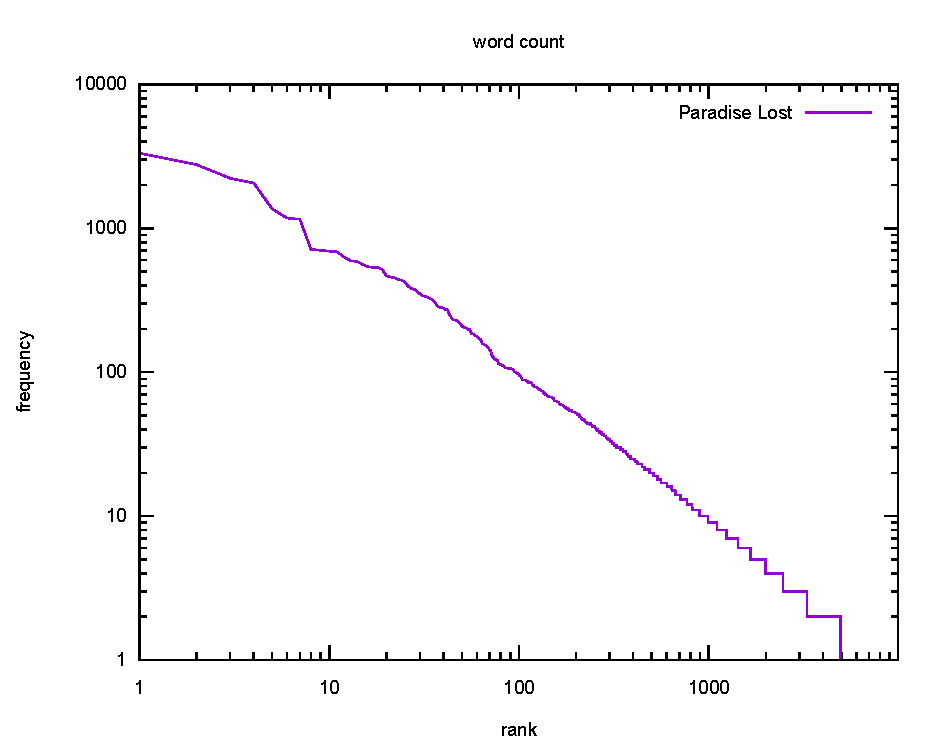
\includegraphics[width=0.75\textwidth]{imgs/wordcound.pdf}
\caption{Frequency of occurrence of words in \textit{Paradise Lost}.}
\end{figure}

\section{Couting words}\label{sec-count}
\lipsum[2]
Blabla section \ref{sec-intro}.

\lipsum[3][1-3]

\lstinputlisting[language=Bash, firstline=21, lastline=24, 
    breaklines=true, basicstyle=\linespread{1}\small\ttfamily, showstringspaces=false, 
    caption={Using GNUplot to create a log-log plot of rank vs frequency of occurrence of words for the book \textit{Paradise Lost}.}]{./src/paradiselost.sh}

\printbibliography
\end{document}
